\documentclass{beamer} 
\usepackage{beamerthemeshadow}
\usepackage[latin1]{inputenc}
\usepackage[brazil]{babel}
\usepackage{graphicx}
\usepackage{listings}
\title[]{Uso de AMQP para Transporte de Mensagens entre Atores Remotos} 
\author{Thadeu de Russo e Carmo \\ \texttt{thadeurc@ime.usp.br}} 
\institute{Orientador: Prof. Dr. Francisco da Rocha Reverbel\\ Instituto de Matem\'atica e Estat\'istica \\ Universidade de S\~ao Paulo}
\date{Dezembro, 2010}

\begin{document}
\frame{\titlepage}
\section{Introdu\c{c}\~ao} 
\frame{\frametitle{Proposta}
    	\only<1>{
     		Explorar a potencial sinergia entre duas classes de sistemas de \textit{software}:
 		\begin{enumerate}
 			\item Sistemas corporativos: composta de sistemas de \textit{middleware} orientados a mensagens e 
				\textit{message brokers}
			\item Programas concorrentes: composta pelas implementa\c{c}\~oes do modelo de atores
 		\end{enumerate}
	}
}
\frame{
\frametitle{Motiva\c{c}\~ao -- Sistemas corporativos}
	\only<1>{
		\begin{itemize}
			\item \textit{Middlewares} orientados a mensagem (MOMs) trabalham com troca ass\'incrona de mensagens
			\item Formam base para simplificar o desenvolvimento de sistemas
			\item Possuem suporte e mecanismos para gerenciamento robusto de erros e garantia de entrega de mensagens	
			\item S\~ao frequentemente apresentados como tecnologia que pode mudar a maneira como sistemas distribu\'idos
			s\~ao constru\'idos \cite{Alonso2004}
		\end{itemize}
	}
	\only<2>{
         	MOMs s\~ao um tanto quanto inflex\'iveis em rela\c{c}\~ao a filtragem e roteamento de mensagens.		
	}
	\only<3>{
 		\textit{Message brokers} s\~ao descendentes diretos diretos de MOMs que endere\c{c}\~ao essas limita\c{c}\~oes.		
	}
	\only<4>{
 		Os protocolos usados por \textit{message brokers} variam de produto para produto. Algumas abordagens existentes:
 		\begin{itemize}
 			\item A especifica\c{c}\~ao Java \textit{Message Service} (JMS) define uma API padr\~ao para que programas Java possam
			interagir com \textit{message brokers}
 			\item A especifica\c{c}\~ao \textit{Advanced Message Queuing Protocol}(AMQP) \'e uma proposta
 			recente de padroniza\c{c}\~ao de um protocolo para \textit{message brokers}
 		\end{itemize}
	}
}
\frame{
\frametitle{Motiva\c{c}\~ao -- Programas concorrentes}

	\only<1>{
		Processadores \textit{multicore} impactam a maneira que programas s\~ao escritos:
		\begin{itemize}
			\item  Programas precisam ser escritos de maneira concorrente para poder
			usufruir dos ganhos de desempenho dos processadores com m\'ultiplos n\'ucleos \cite{Sutter2005}
			
			\item Abordagem convencional com o uso de travas al\'em de complexa, possui
			limita\c{c}\~oes em rela\c{c}\~ao a componibilidade \cite{Jones2007}

			\item A maioria das linguagems de programa\c{c}\~ao n\~ao s\~ao adequadas para a cria\c{c}\~ao de tais
			programas \cite{SutterEtAll2005}
		\end{itemize}
	}
	\only<2>{
		Modelos n\~ao convencionais de programa\c{c}\~ao concorrente:
		\begin{itemize}
			\item \textit{Software Transactional Memory} (STM) -- mecanismo de controle an\'alogo
			\`as transa\c{c}\~oes de bancos de dados
			\item Atores -- troca de mensagem ass\'incrona entre processos 
		\end{itemize}
	}
	\only<3>{
		\begin{beamerboxesrounded}{Defini\c{c}\~ao de um Ator \cite{Agha1986}}
			\'E um agente computacional que possui uma caixa de correio e um comportamento.
			Atores processam assicronamente as mensagens recebidas em suas respectivas caixas de correios. 
			As mensagens recebidas s\~ao mapeadas em uma $3$-tupla consistindo de: 
			\begin{itemize}
				\item Um conjunto finito de mensagens enviadas para outros atores onde o endere\c{c}o \'e conhecido
				(incluindo o pr\'oprio ator que est\'a processando a mensagem)
				\item Um novo comportamento a ser usado no processamento a mensagem seguinte
				\item Um conjunto finito de cria\c{c}\~ao de novos atores
			\end{itemize}
		\end{beamerboxesrounded}
	}
}
\frame{
\frametitle{Motiva\c{c}\~ao}
	\only<1>{
		Potencial sinergia em as duas classes:
		\begin{itemize}
			\item Atores em diferentes n\'os podem trocar mensagens entre si
			\item \textit{Message brokers} prov\^em robustes para a troca de mensagens entre entidades em diferentes n\'os de um sistema
		\end{itemize}
	}
}
\frame{\frametitle{Objetivos}
	O principal objetivo deste trabalho \'e gerar um prot\'otipo baseado na implementa\c{c}\~ao de atores do projeto 
	Akka, que utilize um \textit{message broker} AMQP para o transporte das mensagens entre atores remotos.
}

\section{Trabalhos Relacionados}
\subsection{Atores em Erlang}
\frame{
\frametitle{Atores em Erlang}
	\begin{beamerboxesrounded}{Principais caracter\'isticas}
		\begin{itemize}
			\item Atores s\~ao processos ultra leves criados dentro da m\'aquina virtual Erlang
			\item Primitivas para cria\c{c}\~ao de novos atores (\textit{spawn}), envio de mensagens (!), 
			recebimento (\textit{receive}) e cria\c{c}\~ao de hieraquia de supervis\~ao (\textit{link}) est\~ao
			embutidos na linguagem
			\item \textit{Spawns} remotos s\~ao poss\'iveis e o transporte das mensagens \'e feito com o uso
			de \textit{sockets} TCP e UDP
			\item Mensagens que n\~ao est\~ao definidas no comportamento do ator s\~ao recolocadas na 
			caixa de correio do ator para tentativa de processamento futuro
		\end{itemize}
	\end{beamerboxesrounded}
}
\subsection{Atores em Scala}
\frame{
\frametitle{A biblioteca de atores de Scala}
	\only<1>{A implementa\c{c}\~ao da biblioteca padr\~ao de Scala foi baseada na implementa\c{c}\~ao feita em Erlang, possuindo
	basicamente as mesmas funcionalidades j\'a descritas.
	}
	\only<2>{
		\begin{beamerboxesrounded}{Caracter\'isticas adicionais}
			\begin{itemize}
				\item Atores s\~ao baseados em \textit{threads} Java
				\item Possui m\'etodos como \textit{act} e \textit{react} a serem usados como alternativa ao \textit{receive}, 
				que permitem um reuso de \textit{threads} inativas
			\end{itemize}
		\end{beamerboxesrounded}
	}
	\only<3>{
		\begin{beamerboxesrounded}{Outros tipos de envio}
			\begin{itemize}
				\item !? : faz o envio da mensagem e fica bloqueado dentro de um tempo limite aguardando a resposta
				\item !! : faz o envio da mensagem e recebe um resultado substitudo (\textit{Future}). Uma fun\c{c}\~ao parcial
				fica aguardando o resultado real
			\end{itemize}
		\end{beamerboxesrounded}
		\textit{Future} \'e um mecanismo usado para  retornar valores de chamadas ass\'incronas, e age como um substituto
		para o resultado que ainda n\~ao foi materializado.
	}	
	\only<4>{
		\begin{beamerboxesrounded}{Atores Remotos}
			\begin{itemize}
				\item Cria\c{c}\~ao de atores remotos (\textit{spawn remotes}) n\~ao \'e poss\'ivel
				\item Atores s\~ao acess\'iveis remotamente via \textit{proxies}
				\item Clientes obt\'em refer\^encias para atores remotos s\~ao fazendo buscas em um determinado n\'o 
				(JVM com \textit{host} e porta) utilizando como chave o nome sob o qual o ator foi registrado
				\item O transporte das mensagens \'e feito via seria\c{c}\~ao padr\~ao Java atrav\'es de \textit{sockets} TCP
			\end{itemize}
		\end{beamerboxesrounded}
	}
}
\subsection{O projeto Akka}
\frame{
\frametitle{O projeto Akka}
		\only<1>{
			\'E composto por um conjunto de m\'odulos que juntos formam uma plataforma voltada para o desenvolvimento
			de aplica\c{c}\~oes escal\'aveis e tolerante a falhas.
		}
		\only<2>{
			\begin{beamerboxesrounded}{Principais m\'odulos}
				\begin{itemize}
					\item Atores locais
					\item Atores remotos
					\item STM
					\item Hierarquia de supervis\~ao
					\item \textit{Transactors} (combina\c{c}\~ao de atores com STM)
				\end{itemize}
			\end{beamerboxesrounded}
			Al\'em de m\'odulos adicionais para integra\c{c}\~ao com outras tecnologias.
		}
}
\section{Advanced Message Queuing Protocol}
\frame{
\frametitle{Advanced Message Queuing Protocol}
	\only<1>{
		\begin{itemize}
			\item Protocolo aberto desenvolvido por um conjunto de empresas com o objetivo de padroniza\c{c}\~ao
			e redu\c{c}\~ao de custos na integra\c{c}\~ao de sistemas
			\item Al\'em da defini\c{c}\~ao do protocolo, define tamb\'em a sem\^antica dos servidos da aplica\c{c}\~ao servidora 
			\item Objetiva que as capacidades de MOMs estejam dispon\'iveis pervasivamente nas empresas
		\end{itemize}
	}
	\only<2>{
		\begin{beamerboxesrounded}{Principais componentes}
			\begin{itemize}
				\item Servidor, tamb\'em conhecido como \textit{broker}
				\item Filas
				\item \textit{Exchanges}
				\item \textit{Bindings}
				\item \textit{Virtual hosts}
			\end{itemize}
		\end{beamerboxesrounded}
		Sistemas AMQP o recebimendo e roteamento das mensagens s\~ ao separados do seu armazemento
		e encaminhamento. Em sistemas pr\'e-AMQP, estas tarefas s\~ao feitas por blocos monol\'iticos.
	}
	\only<3>{
		\begin{figure}[hbtp]
			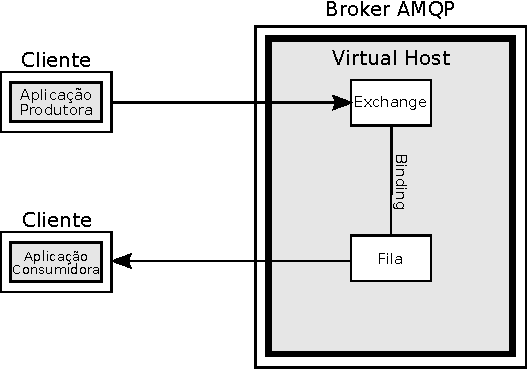
\includegraphics[scale=.85]{imagens/amqp-overview.pdf}
		\end{figure}
	}
	\only<4>{
		\begin{figure}[hbtp]
			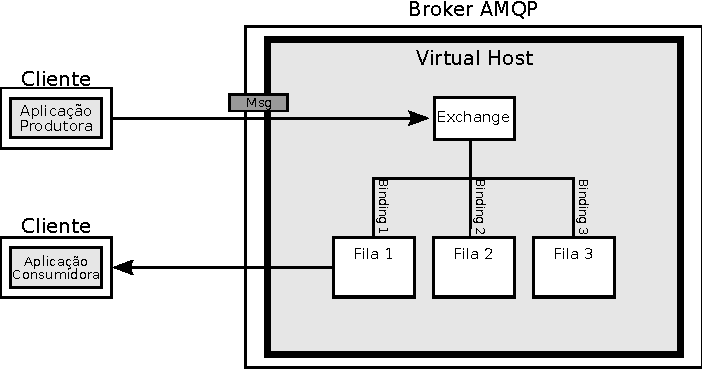
\includegraphics[scale=.90]{imagens/amqp-message-flow1.pdf}
		\end{figure}
	}
	\only<5>{
		\begin{figure}[hbtp]
			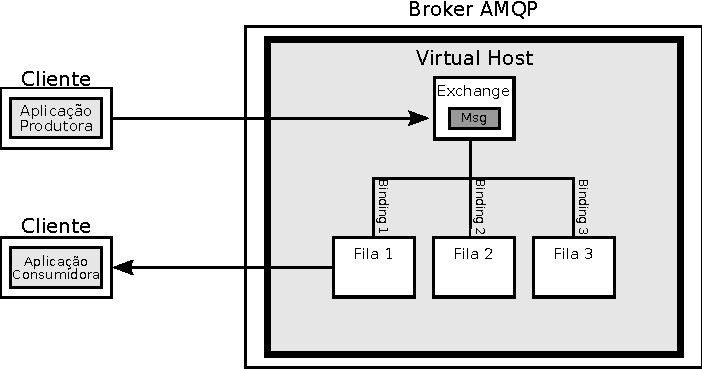
\includegraphics[scale=.90]{imagens/amqp-message-flow2.pdf}
		\end{figure}
	}
	\only<6>{
		\begin{figure}[hbtp]
			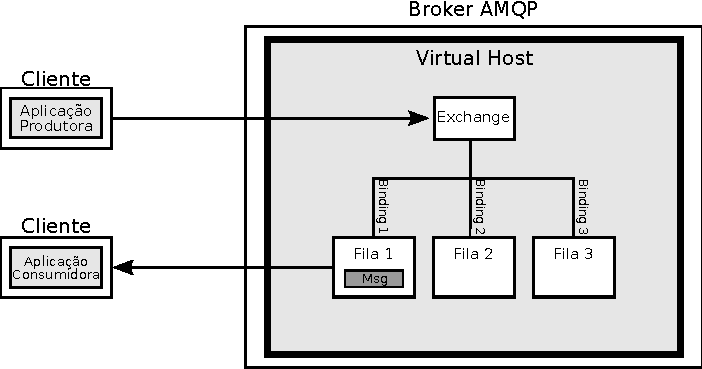
\includegraphics[scale=.90]{imagens/amqp-message-flow3.pdf}
		\end{figure}
	}
	\only<7>{
		\begin{beamerboxesrounded}{Analogia com sistemas de correio eletr\^onico}
			\begin{itemize}
				\item Mensagens AMQP s\~ao an\'alogas a mensagens de correio eletr\^onico
				\item Filas s\~ao an\'alogas a caixas de correio
				\item \textit{Exchanges} s\~ao an\'alogas a agentes de transfer\^encia de mensagens (MTA), e
				com base nas chaves de roteamento (To, Cc e Bcc no caso de correio eletr\^onico), verifica
				as tabelas de registro e decide como enviar as mensagens para uma ou mais caixas de correio
				\item \textit{Bindings} correspondem a entradas nas tabelas de roteamento do MTA		
			\end{itemize}
		\end{beamerboxesrounded}
	}
}

\section{Atores no projeto Akka}
\frame{
\frametitle{Atores no projeto Akka}
	\only<1>{
		A implementa\c{c}\~ao da biblioteca \'e totalmente independente da biblioteca de atores presente na distrubui\c{c}\~ao da linguagem Scala,
	 	e tamb\'em foi baseada na implementa\c{c}\~ao feita em Erlang.
	}
	\only<2>{
		\begin{beamerboxesrounded}{Principais caracter\'isticas}
			\begin{itemize}
				\item Tipos adicionais de envio (!! e !!!), semelhantes a !? e !!
				\item Diferentes tipos de despachadores de mensagem
				\item \textit{Remote spawns}, mas sem carregamento remoto de classes
				\item Transporte de mensagens via \textit{sockets} TCP com aux\'ilio do JBoss Netty
				\item Direfentes protocolos para seria\c{c}\~ao de mensagens em envios para atores remotos
				(Protobuf, JSON, seria\c{c}\~ao Java padr\~ao, SBinary)
				\item Compacta\c{c}\~ao das mensagens enviadas para atores remotos (JBoss Netty)
			\end{itemize}
		\end{beamerboxesrounded}
	}
	\only<3>{
 		\begin{beamerboxesrounded}{Ator Local e Ator Remoto}
			\begin{itemize}
				\item Ator local: \'e um ator que pode receber mensagens apenas de atores residentes na mesma m\'aquina
				virtual
				\item Ator remoto (ou ator remotamente acess\'ivel): \'e um ator que pode receber mensagens de quaisquer outros atores, inclusive os
				residentes em outras m\'aquinas virtuais 
			\end{itemize}
			
		\end{beamerboxesrounded}
	}
}
\subsection{Atores locais}
\begin{frame}[fragile]
\frametitle{Envio local de mensagens}
\begin{verbatim}
import se.scalablesolutions.akka.actor.Actor._

class MyActor extends Actor {
  def receive = {
    case "test" => println("received test")
    case      _ => println("received unknown message")
  }
}
	    
val myActor = actorOf[MyActor].start
myActor ! "test"
\end{verbatim}
\end{frame}
\frame{
	\only<1>{
		\begin{figure}[hbtp]
			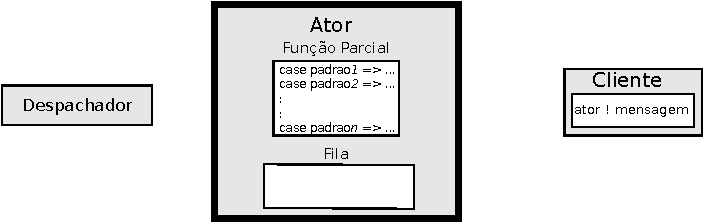
\includegraphics[scale=.9]{imagens/local-actor-message1.pdf}
		\end{figure}
	}
	\only<2>{
		\begin{figure}[hbtp]
			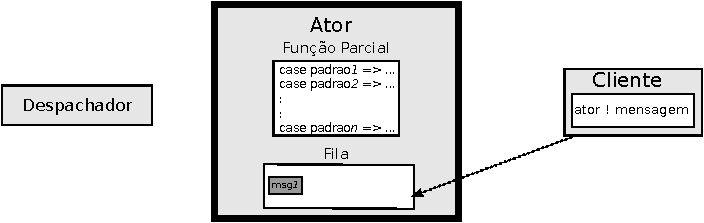
\includegraphics[scale=.9]{imagens/local-actor-message2.pdf}
		\end{figure}
	}
	\only<3>{
		\begin{figure}[hbtp]
			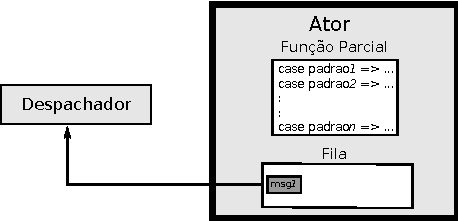
\includegraphics[scale=.9]{imagens/local-actor-message3.pdf}
		\end{figure}
	}
	\only<4>{
		\begin{figure}[hbtp]
			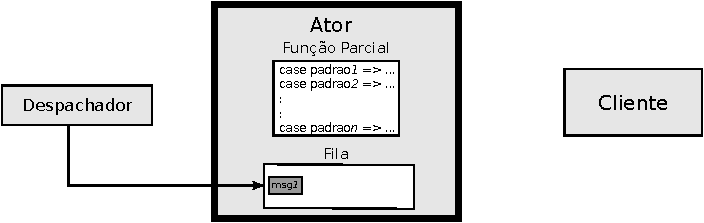
\includegraphics[scale=.9]{imagens/local-actor-message3_1.pdf}
		\end{figure}
	}
	\only<5>{
		\begin{figure}[hbtp]
			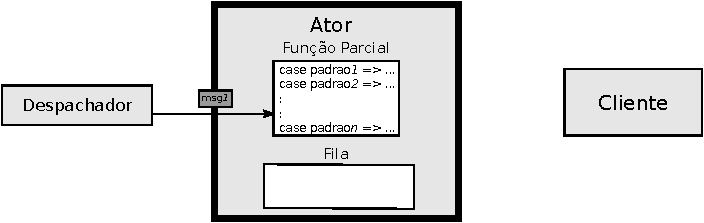
\includegraphics[scale=.9]{imagens/local-actor-message4.pdf}
		\end{figure}
	}

}

\subsection{Atores remotos}
\frame{
\frametitle{Principais componentes}
	\only<1>{
		\begin{beamerboxesrounded}{Principais componentes}
			\begin{itemize}
				\item \textit{RemoteActor}
				\item \textit{RemoteServer}
				\item \textit{RemoteNode}
				\item \textit{Cluster}
				\item \textit{RemoteClient}
			\end{itemize}
		\end{beamerboxesrounded}
	}
	\only<2>{
		\begin{figure}[hbtp]
			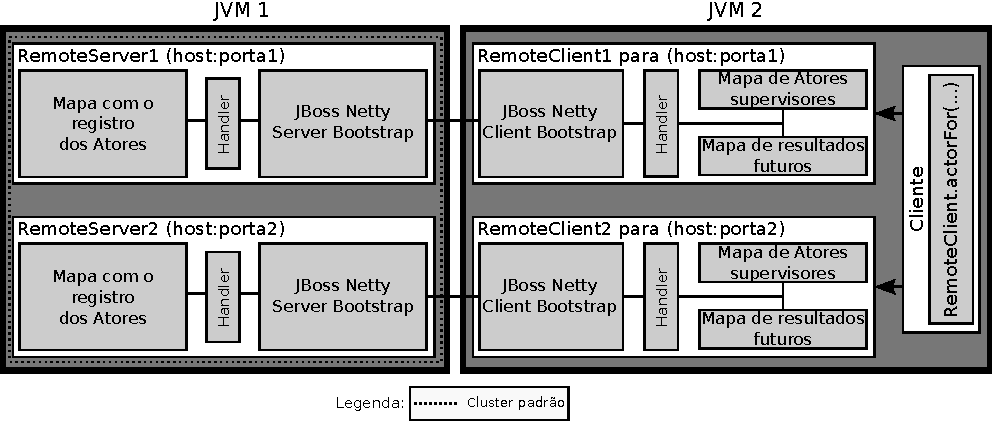
\includegraphics[scale=.6]{imagens/remote-actor-diagram.pdf}
		\end{figure}
	}
}
\begin{frame}[fragile]
\frametitle{Envio remoto de mensagens}
	\begin{itemize}
		\item Cria\c{c}\~ao de ator remoto pelo cliente:
	\end{itemize}
	\begin{verbatim}
	   val myActor = actorOf[MyActor]
	   myActor.makeRemote("localhost", 15092)
	   myActor.start
	   myActor ! "test"
	\end{verbatim}
\end{frame}
\begin{frame}[fragile]
\frametitle{Envio remoto de mensagens}
	\begin{itemize}
		\item Registro de um ator local para receber mensagens de atores remotos:
	\begin{verbatim}
		RemoteNode.start("localhost", 15092)
		RemoteNode.register("my-actor", myActor)
	\end{verbatim}
	\item Cliente enviando mensagem para o ator remoto:
	\begin{verbatim}
		val myActor = RemoteClient.actorFor("my-actor", 
                                 "localhost", 15092)
		myActor ! "Hi"
	\end{verbatim}
	\end{itemize}
\end{frame}

\frame{
	\only<1>{
		\begin{figure}[hbtp]
			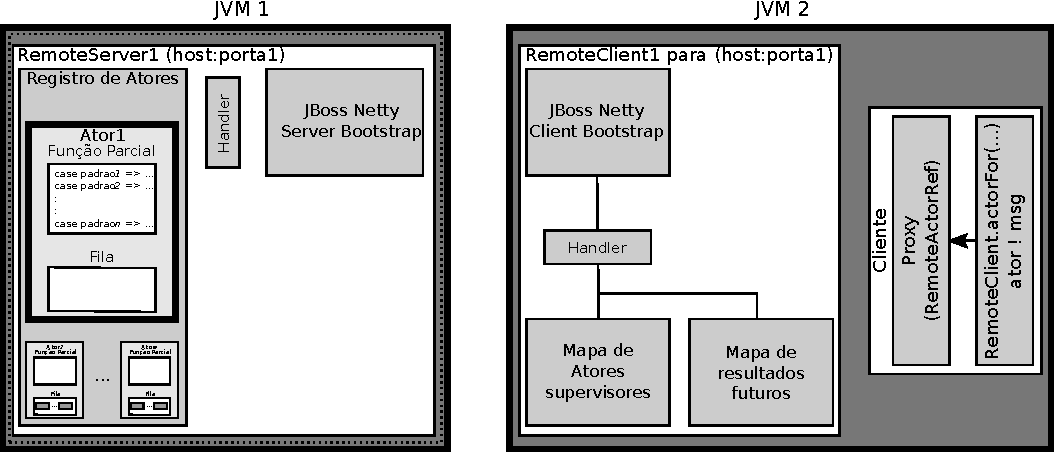
\includegraphics[scale=.6]{imagens/remote-actor-message-flow1.pdf}
		\end{figure}
	}
	\only<2>{
		\begin{figure}[hbtp]
			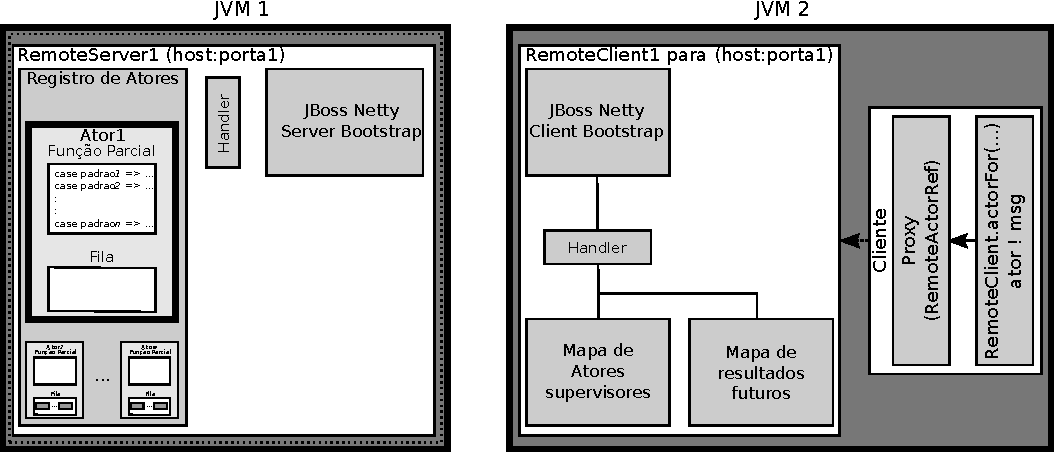
\includegraphics[scale=.6]{imagens/remote-actor-message-flow2.pdf}
		\end{figure}
	}
	\only<3>{
		\begin{figure}[hbtp]
			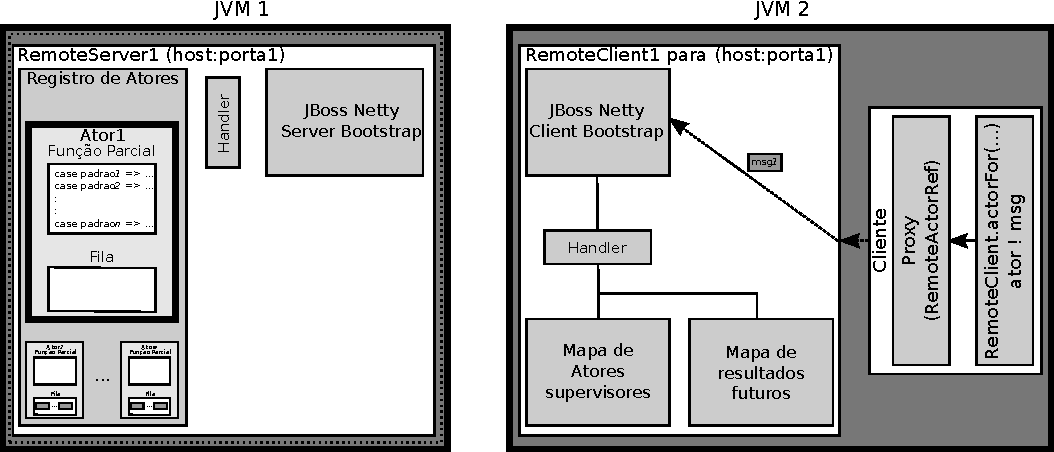
\includegraphics[scale=.6]{imagens/remote-actor-message-flow3.pdf}
		\end{figure}
	}
	\only<4>{
		\begin{figure}[hbtp]
			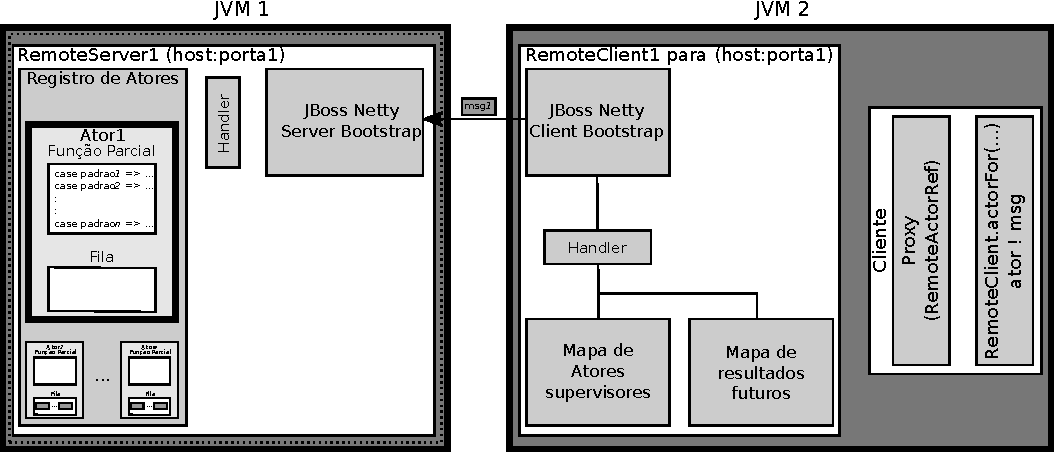
\includegraphics[scale=.6]{imagens/remote-actor-message-flow4.pdf}
		\end{figure}
	}
	\only<5>{
		\begin{figure}[hbtp]
			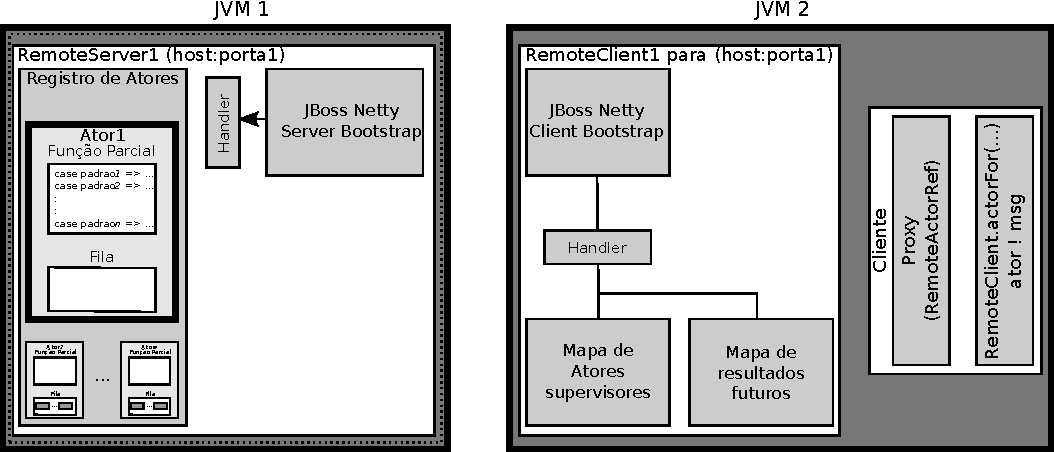
\includegraphics[scale=.6]{imagens/remote-actor-message-flow5.pdf}
		\end{figure}
	}
	\only<6>{
		\begin{figure}[hbtp]
			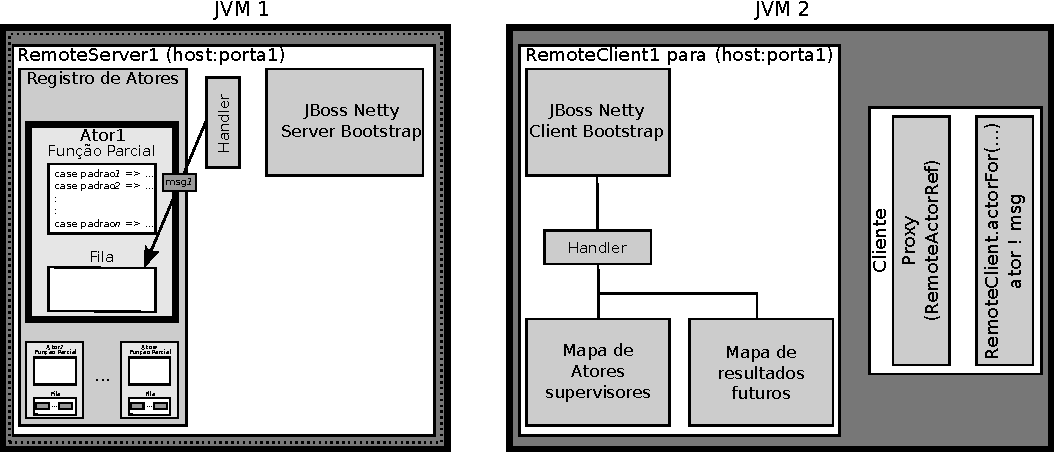
\includegraphics[scale=.6]{imagens/remote-actor-message-flow6.pdf}
		\end{figure}
	}
	\only<7>{
		\begin{figure}[hbtp]
			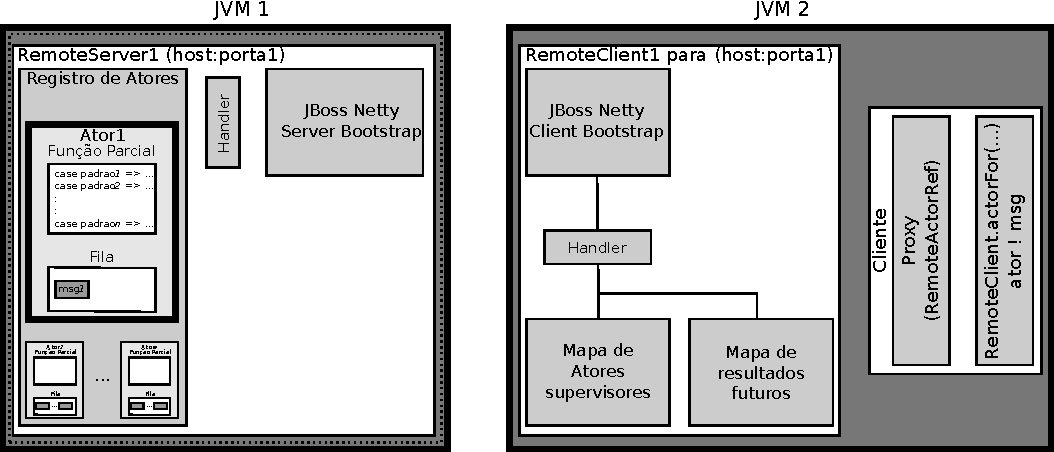
\includegraphics[scale=.6]{imagens/remote-actor-message-flow7.pdf}
		\end{figure}
	}
}
\section{O projeto} 
\frame{
\frametitle{O projeto}
	\only<1>{
 		A implementa\c{c}\~ao do modelo de atores do projeto Akka \'e mais abrangente e robusta do que a implenta\c{c}\~ao
		presente na distribui\c{c}\~ao da linguagem Scala, em particular para atores remotos.
	}
	\only<2>{
		Criar uma vers\~ao modificada do Akka, na qual o envio de mensagens para atores remotos seja feito via AMQP.
	}
}
\subsection{Atividades programadas}
\frame{
\frametitle{Cronograma}
	\only<1>{
		\begin{enumerate}
			\item An\'alise das implementa\c{c}\~oes dos \textit{brokers} AMQP para 
			defini\c{c}\~ao do que ser\'a usado
			\item An\'alise e desenvolvimento do c\'odigo e estrutura necess\'aria para o transporte
			 das mensagens entre os atores remotos utilizando AMQP
			\item Desenvolvimento de testes, refatora\c{c}\~ao e aprimoramento da implementa\c{c}\~ao
			\item Elabora\c{c}\~ao e execu\c{c}\~ao cen\'arios de experimento para compara\c{c}\~ao entre a vers\~ao
			original do Akka e a vers\~ao a ser desenvolvida
			\item Reda\c{c}\~ao da disserta\c{c}\~ao
			\item Reda\c{c}\~ao de artigo
			\item Defesa
		\end{enumerate}
	}
	\only<2>{
		\begin{center}	
		\newcommand{\x}{$\bullet$}
			\textbf{2010/2011}		  
			\begin{tabular}{|c|c|c|c|c|c|c|c|c|c|c|c|c|c|}
			 \hline
			 & nov & dez & jan & fev & mar & abr & mai & jun & jul \\ \hline
			    1 & \x  &     &     &     &     &     &     &     &     \\ \hline
			    2 &     & \x  & \x  & \x  &     &     &     &     &     \\ \hline
			    3 &     &     & \x  & \x  & \x  &     &     &     &     \\ \hline
			    4 &     &     &     &     & \x  & \x  &     &     &     \\ \hline
			    5 &     &     &     &     & \x  & \x  & \x  & \x  &     \\ \hline
			    6 &     &     &     &     &     &     &     & \x  & \x    \\ \hline
			    7 &     &     &     &     &     &     &     &     & \x  \\ \hline
		  	\end{tabular}  
		\end{center}	
		\begin{center}
			\vspace{.5cm}
			Data limite: Fevereiro de 2012.
		\end{center}
	}
}
\subsection{Refer\^encias}
\frame{
\frametitle{Refer\^encias}
\begin{thebibliography}{10} 
	\only<1>{
		\bibitem[Sutter, 2005]{Sutter2005} Herb Sutter, 2005 
		\newblock {\em The Free Lunch Is Over: A Fundamental Turn Toward Concurrency in Software}
		\newblock http://www.gotw.ca/publications/concurrency-ddj.htm
	
		\bibitem[Sutter, Larus. 2005]{SutterEtAll2005} Herb Sutter and James Larus. 2005
		\newblock {\em Software and the Concurrency Revolution}
		\newblock ACM Queue 3(7): 54 -62
	}
	\only<2>{
		\bibitem[Agha, 1986]{Agha1986} Gul Agha, 1986 
		\newblock {\em Actors: a model of concurrent computation in distributed system}
		\newblock MIT Press, Cambridge, MA, USA
	
		\bibitem[Jones, 2007]{Jones2007} Simon P. Jones, 2007
		\newblock {\em Beautiful Concurrency}
		\newblock http://research.microsoft.com/Users/simonpj/papers/stm/index.htm
 	
	}
	\only<3>{
		\beamertemplatebookbibitems
		\bibitem[Alonso, et al. 2004]{Alonso2004} Gustavo Alonso and Fabio Casati and Harumi Kuno and Vijay Machiraju, 2004
		\newblock {\em Web Services: Concepts, Architecture and Applications}
	}
\end{thebibliography}
}
\subsection{Perguntas}
\frame{
\frametitle{Perguntas}
	\begin{figure}[hbtp]
		
\includegraphics[scale=0.5]{imagens/question.pdf}
	\end{figure}
}


\end{document}
